\ifx\wholebook\relax \else

\documentclass[b5paper]{article}
\usepackage[nomarginpar
  %, margin=.5in
]{geometry}

\addtolength{\oddsidemargin}{-0.05in}
\addtolength{\evensidemargin}{-0.05in}
\addtolength{\textwidth}{0.1in}

\usepackage[en]{../../../prelude}

\setcounter{page}{1}

\begin{document}

\title{AVL tree}

\author{Xinyu LIU
\thanks{{\bfseries Xinyu LIU} \newline
  Email: liuxinyu95@gmail.com \newline}
  }

\maketitle
\fi

\markboth{AVL tree}{Elementary Algorithms}

\ifx\wholebook\relax
\chapter{AVL tree}
\numberwithin{Exercise}{chapter}
\fi

\section{Introduction}
\label{introduction} \index{AVL tree}

The idea of red-black tree is to limit the number nodes along a path within a range. AVL tree takes a direct approach: quantify the difference between branches. For a node $T$, define:

\be
  \delta(T) = |r| - |l|
\ee

Where $|T|$ is the height of tree $T$, $l$ and $r$ are the left and right sub-trees. Define $\delta(\nil) = 0$ for the empty tree. If $\delta(T) = 0$ for every node $T$, the tree is definitely balanced. For example, a complete binary tree has $n=2^h - 1$ nodes for height $h$. There are not any empty branches unless the leaves. The less absolute value of $\delta(T)$, the more balanced between the sub-trees. We call $\delta(T)$ the {\em balance factor} of a binary tree.

\section{Definition}
\index{AVL tree!definition}

\begin{figure}[htbp]
   \centering
   \includegraphics[scale=0.5]{img/avl-example.ps}
   \caption{an AVL tree}
   \label{fig:avl-example}
\end{figure}

A binary search tree is an AVL tree if every sub-tree $T$ satisfies:

\be
  |\delta(T)| \leq 1
  \label{eq:avl-rule}
\ee

There are three valid values for $\delta(T)$: $\pm 1$, and 0. Figure \ref{fig:avl-example} shows an AVL tree. This definition ensures the tree height $h = O(\lg n)$, where $n$ is the number of nodes in the tree. Let's prove it. For an AVL tree of height $h$, the number of nodes varies. There are at most $2^h - 1$ nodes for a complete binary tree case. We are interesting in how many nodes at least. Let the minimum number be $N(h)$. We have the following result:

\begin{itemize}
\item Empty tree $\nil$: $h = 0$, $N(0) = 0$;
\item Singleton tree: $h = 1$, $N(1) = 1$;
\end{itemize}

Figure \ref{fig:N-h-relation} shows an AVL tree $T$ of height $h$. It contains three parts, the key $k$, and two sub-trees $l$, $r$. We have the following equation:

\begin{figure}[htbp]
   \centering
   \includegraphics[scale=0.5]{img/Nh-lvr.ps}
   \caption{An AVL tree of height $h$. The height of one sub-tree is $h-1$, the other is no less than $h-2$.}
   \label{fig:N-h-relation}
\end{figure}

\be
  h = max(|l|, |r|) + 1
\ee

There must be a sub-tree of height $h - 1$. From the definition. we have $||l|-|r|| \leq 1$ holds. Hence the height of the other tree can not be lower than $h - 2$. The total number of the nodes in $T$ is the sum of both sub-trees plus 1 (for the root):

\be
  N(h) = N(h-1) + N(h-2) + 1
  \label{eq:Fibonacci-like}
\ee

This recursive equation is similar to Fibonacci numbers. Actually we can transform it to Fibonacci numbers through $N'(h) = N(h) + 1$. Equation (\ref{eq:Fibonacci-like}) then changes to:

\be
  N'(h) = N'(h-1) + N'(h-2)
\ee

\begin{lemma}
\label{lemma:N-phi}
Let $N(h)$ be the minimum number of nodes for an AVL tree of height $h$, and $N'(h) = N(h) + 1$, then
\be
  N'(h) \geq \phi^h
\ee

Where $\phi = \dfrac{\sqrt{5}+1}{2}$ is the golden ratio.
\end{lemma}

\begin{proof}
When $h = 0$ or 1, we have:
\begin{itemize}
\item $h = 0$: $N'(0) = 1 \geq \phi^0 = 1$
\item $h = 1$: $N'(1) = 2 \geq \phi^1 = 1.618...$
\end{itemize}

For the induction case, assume $N'(h) \geq \phi^h$.
\[
  \begin{array}{rll}
  N'(h+1) & = N'(h) + N'(h-1) & \{\text{Fibonacci}\} \\
          & \geq \phi^h + \phi^{h-1} & \\
          & = \phi^{h-1}(\phi + 1) & \{\phi + 1 = \phi^2 = \dfrac{\sqrt{5}+3}{2}\} \\
          & = \phi^{h+1}
 \end{array}
\]
\end{proof}

From Lemma \ref{lemma:N-phi}, we immediately obtain:

\be
  h \leq log_{\phi}(n+1) = log_{\phi}2 \cdot \lg (n+1) \approx 1.44 \lg (n+1)
  \label{eq:AVL-height}
\ee

We prove the height of AVL tree is proportion to $O(\lg n)$, indicating AVL tree is balanced.

When insert or delete, the balance factor may exceed the valid value range, we need fix to resume $|\delta|<1$. Traditionally, the fixing is through tree rotations. We give the simplified implementation based on pattern matching. The idea is similar to the functional red-black tree(Okasaki, \cite{okasaki}). Because of this `modify-fix' approach, AVL tree is also self-balanced binary search tree. We can re-use the binary search tree definition. Although the balance factor $\delta$ can be computed recursively, we record it inside each node as $T = (l, k, r, \delta)$, and update it when mutate the tree\footnote{Alternatively, we can record the height instead of $\delta$\cite{py-avl}.}. Below example program adds $\delta$ as an \texttt{Int}:

\lstset{frame = single}
\begin{Haskell}
data AVLTree a = Empty
               | Br (AVLTree a) a (AVLTree a) Int
\end{Haskell}

For AVL tree, $lookup$, $max$, $min$ are as same as the binary search tree. We focus on $insert$ and $delete$ algorithms.

\section{Insert}
\index{AVL tree!insert}

When insert a new element, $|\delta(T)|$ may exceed 1. We can use pattern matching similar to red-black tree to develop a simplified solution. After insert element $x$, for those sub-trees which are the ancestors of $x$, the height may increase at most by 1. We need recursively update the balance factor along the path of insertion. Define the insert result as a pair $(T', \Delta H)$, where $T'$ is the updated tree and $\Delta H$ is the increment of height. We modify the binary search tree $insert$ function as below:

\be
insert = \textit{fst} \circ ins
\ee

Where $\textit{fst}\ (a, b) = a$ returns the first element in a pair. $ins(T, k)$ does the actual work to insert element $k$ into tree $T$:

\be
\begin{array}{rcl}
ins\ \nil\ k & = & ((\nil, k, \nil, 0), 1) \\
ins\ (l, k', r, \delta)\ k & = & \begin{cases}
  k < k': tree\ (ins\ l\ k)\ k'\ (r, 0)\ \delta \\
  k > k': tree\ (l, 0)\ k'\ (ins\ r, k)\ \delta \\
\end{cases}
\end{array}
\label{eq:ins}
\ee

If the tree is empty $\nil$, the result is a leaf of $k$ with balance factor 0. The height increases to 1. Otherwise let $T = (l, k', r, \delta)$. We compare the new element $k$ with $k'$. If $k < k'$, we recursively insert $k$ it to the left sub-tree $l$, otherwise insert to $r$. As the recursive insert result is a pair of $(l', \Delta l)$ or $(r', \Delta r)$, we need adjust the balance factor and update tree height through function $tree$, it takes 4 parameters: $(l', \Delta l)$, $k'$, $(r', \Delta r)$, and $\delta$. The result is $(T', \Delta H)$, where $T'$ is the new tree, and $\Delta H$ is defined as:

\be
  \Delta H = |T'| - |T|
\ee

We can further break it down into 4 cases:

\be
\begin{array}{rcl}
  \Delta H & = & |T'| - |T| \\
           & = & 1 + max(|r'|, |l'|) - (1 + max(|r|, |l|)) \\
           & = & max(|r'|, |l'|) - max(|r|, |l|) \\
           & = & \begin{cases}
\delta \geq 0, \delta' \geq 0: & \Delta r \\
\delta \leq 0, \delta' \geq 0: & \delta + \Delta r \\
\delta \geq 0, \delta' \leq 0: & \Delta l - \delta \\
otherwise: & \Delta l
\end{cases}
\end{array}
\ee

Where $\delta' = \delta(T') = |r'| - |l'|$, is the updated balance factor. Appendix B provides the proof for it. We need determine $\delta'$ before balance adjustment.

\be
\begin{array}{rcl}
\delta' & = & |r'| - |l'| \\
        & = & |r| + \Delta r - (|l| + \Delta l) \\
        & = & |r| - |l| + \Delta r - \Delta l \\
        & = & \delta + \Delta r - \Delta l \\
\end{array}
\ee

With the changes in height and balance factor, we can define the $tree$ function in (\ref{eq:ins}):

\be
tree\ (l', \Delta l)\ k\ (r', \Delta r)\ \delta =
  balance\ (l', k, r', \delta')\ \Delta H
\ee

Below example programs implements what we deduced so far:

\begin{Haskell}
insert t x = fst $ ins t where
    ins Empty = (Br Empty x Empty 0, 1)
    ins (Br l k r d)
        | x < k = tree (ins l) k (r,  0) d
        | x > k = tree (l,  0) k (ins r) d

tree (l, dl) k (r, dr) d = balance (Br l k r d') deltaH where
    d' = d + dr - dl
    deltaH | d >=0 && d' >=0 = dr
           | d <=0 && d' >=0 = d+dr
           | d >=0 && d' <=0 = dl - d
           | otherwise = dl
\end{Haskell}

\subsection{Balance}
\index{AVL tree!balance}
There are 4 cases need fix as shown in figure \ref{fig:avl-insert-fix}. The balance factor is $\pm 2$, exceeds the range of $[-1, 1]$. We adjust them to a uniformed structure in the center, with the $\delta(y) = 0$.

\begin{figure}[htbp]
  \centering
  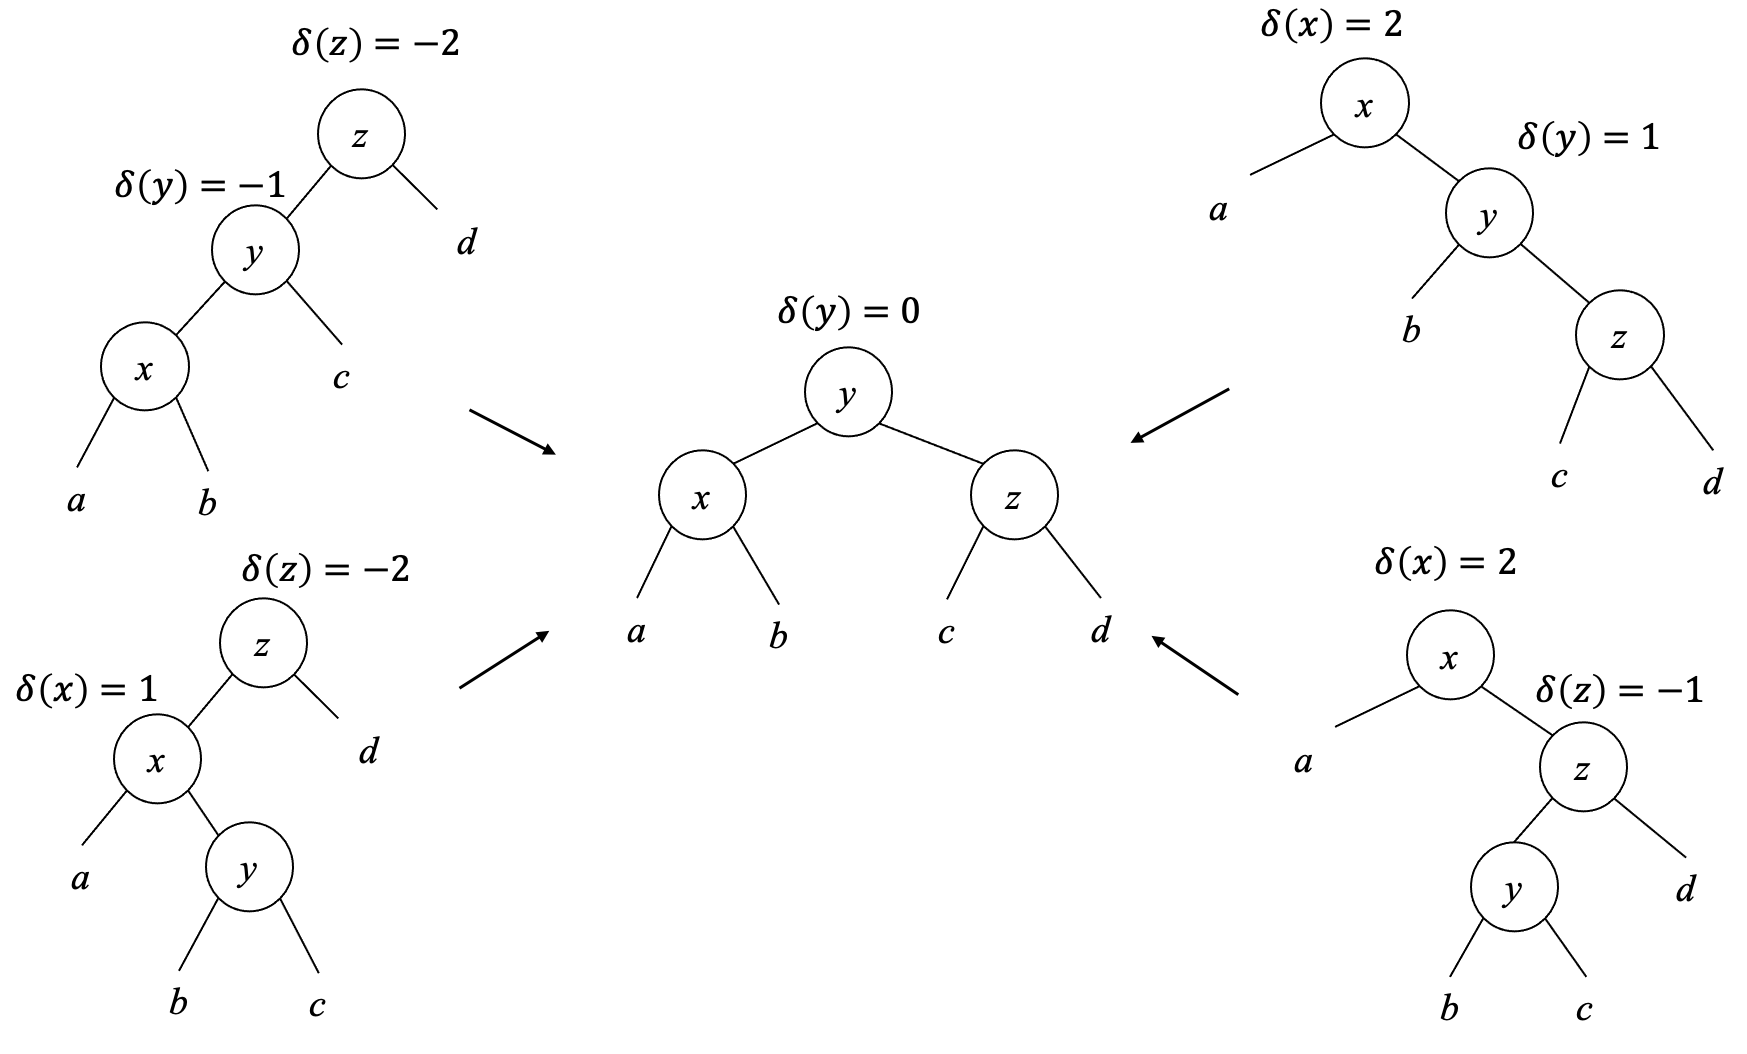
\includegraphics[scale=0.4]{img/avl-insert-fix.png}
  \caption{Fix 4 cases to the same structure}
  \label{fig:avl-insert-fix}
\end{figure}

We call the 4 cases: left-left, right-right, right-left, and left-right. Denote the balance factors before fixing as $\delta(x), \delta(y)$, and $\delta(z)$; after fixing, they change to $\delta'(x), \delta'(y) = 0$, and $\delta'(z)$ respectively. The values of $\delta'(x)$ and $\delta'(z)$ can be given as below. Appendix B gives the proof.

Left-left:

\be
  \begin{array}{l}
  \delta'(x) = \delta(x) \\
  \delta'(y) = 0 \\
  \delta'(z) = 0
  \end{array}
\ee

Right-right:

\be
  \begin{array}{l}
  \delta'(x) = 0 \\
  \delta'(y) = 0 \\
  \delta'(z) = \delta(z)
  \end{array}
  \label{eq:rr-result}
\ee

Right-left and Left-right:

\be
  \begin{array}{l}
  \delta'(x) = \begin{cases}
    \delta(y) = 1: & -1 \\
    otherwise: & 0 \\
    \end{cases} \\
  \delta'(y) = 0 \\
  \delta'(z) = \begin{cases}
    \delta(y) = -1: & 1 \\
    otherwise: & 0 \\
    \end{cases} \\
  \end{array}
  \label{eq:rl-result}
\ee

Based on this, we can implement the pattern matching fix as below:

\be
\resizebox{\textwidth}{!}{\ensuremath{
\begin{array}{rcl}
balance\ (((a, x, b, \delta(x)), y, c, -1), z, d, -2)\ \Delta H & = & ((a, x, b, \delta(x)), y, (c, z, d, 0), 0, \Delta H -1) \\
balance\ (a, x, (b, y, (c, z, d, \delta(z)), 1), 2)\ \Delta H & = & ((a, x, b, 0), y, (c, z, d, \delta(z)), 0, \Delta H -1) \\
balance\ ((a, x, (b, y, c, \delta(y)), 1), z, d, -2)\ \Delta H & = & ((a, x, b, \delta'(x)), y, (c, z, d, \delta'(z)), 0, \Delta H - 1) \\
balance\ (a, x, ((b, y, c, \delta(y)), z, d, -1), 2)\ \Delta H & = & ((a, x, b, \delta'(x)), y, (c, z, d, \delta'(z)), 0, \Delta H - 1) \\
balance\ T\ \Delta H & = & (T, \Delta H) \\
\end{array}
}}
\ee

Where $\delta'(x)$ and $\delta'(z)$ are defined in (\ref{eq:rl-result}). If none of the pattern matches, the last row keeps the tree unchanged. Below is the example program implements $balance$:

\begin{Haskell}
balance (Br (Br (Br a x b dx) y c (-1)) z d (-2)) dH =
            (Br (Br a x b dx) y (Br c z d 0) 0, dH-1)
balance (Br a x (Br b y (Br c z d dz)    1)    2) dH =
            (Br (Br a x b 0) y (Br c z d dz) 0, dH-1)
balance (Br (Br a x (Br b y c dy)    1) z d (-2)) dH =
            (Br (Br a x b dx') y (Br c z d dz') 0, dH-1) where
    dx' = if dy ==  1 then -1 else 0
    dz' = if dy == -1 then  1 else 0
balance (Br a x (Br (Br b y c dy) z d (-1))    2) dH =
            (Br (Br a x b dx') y (Br c z d dz') 0, dH-1) where
    dx' = if dy ==  1 then -1 else 0
    dz' = if dy == -1 then  1 else 0
balance t d = (t, d)
\end{Haskell}

The performance of $insert$ is proportion to the height of the
tree. From (\ref{eq:AVL-height}), it is bound to is $O(\lg n)$ where $n$ is the number of elements in the tree.

\subsubsection{Verification}
\index{AVL tree!verification}
To test an AVL tree, we need verify two things: It is a binary search tree; and for every sub-tree $T$, equation (\ref{eq:avl-rule}): $\delta(T) \leq 1$ holds. Below function examines the height difference between the two sub-trees recursively:

\be
\begin{array}{rcl}
avl?\ \nil & = & \textit{True} \\
avl?\ T & = & avl?\ l\ \land avl?\ r\ \land ||r| - |l|| \leq 1 \\
\end{array}
\ee

Where $l$, $r$ are the left and right sub-trees. The height is calculated recursively:

\be
\begin{array}{rcl}
|\nil| & = & 0 \\
|T| & = & 1 + max(|r|, |l|) \\
\end{array}
\ee

Below example program implements AVL tree height verification:
\begin{Haskell}
isAVL Empty = True
isAVL (Br l _ r _) = isAVL l && isAVL r && abs (height r - height l) <= 1

height Empty = 0
height (Br l _ r _) = 1 + max (height l) (height r)
\end{Haskell}

\begin{Exercise}
\Question{We only give the algorithm to test AVL height. Complete the program to test if a binary tree is AVL tree.}
\end{Exercise}

\section{Imperative AVL tree algorithm $\star$}
\index{AVL tree!imperative insert}

This section gives the imperative algorithm for completeness. Similar to the red-black tree algorithm, we first re-use the binary search tree insert, then fix the balance through tree rotations.

\begin{algorithmic}[1]
\Function{Insert}{$T, k$}
  \State $root \gets T$
  \State $x \gets$ \Call{Create-Leaf}{$k$}
  \State \Call{$\delta$}{$x$} $\gets 0$
  \State $parent \gets$ NIL
  \While{$T \neq$ NIL}
    \State $parent \gets T$
    \If{$k <$ \Call{Key}{$T$}}
      \State $T \gets $ \Call{Left}{$T$}
    \Else
      \State $T \gets $ \Call{Right}{$T$}
    \EndIf
  \EndWhile
  \State \Call{Parent}{$x$} $\gets parent$
  \If{$parent =$ NIL} \Comment{tree $T$ is empty}
    \State \Return $x$
  \ElsIf{$k <$ \Call{Key}{$parent$}}
    \State \Call{Left}{$parent$} $\gets x$
  \Else
    \State \Call{Right}{$parent$} $\gets x$
  \EndIf
  \State \Return \Call{AVL-Insert-Fix}{$root, x$}
\EndFunction
\end{algorithmic}

After insert, the balance factor $\delta$ may change because of the tree growth. Insert to the right may increase $\delta$ by 1, while insert to the left may decrease it. We perform bottom-up fixing from $x$ to root. Denote the new balance factor as $\delta'$, there are 3 cases:

\begin{itemize}
\item $|\delta| = 1$, $|\delta'| = 0$. The new node makes the tree well balanced. The height of the parent keeps unchanged.

\item $|\delta| = 0$, $|\delta'| = 1$. Either the left or the right sub-tree increases its height. We need go on checking the upper level.

\item $|\delta| = 1$, $|\delta'| = 2$. We need rotate the tree to fix the balance factor.
\end{itemize}

\begin{algorithmic}[1]
\Function{AVL-Insert-Fix}{$T, x$}
  \While{\Call{Parent}{$x$} $\neq$ NIL}
    \State $P \gets $ \Call{Parent}{$x$}
    \State $L \gets $ \Call{Left}{$x$}
    \State $R \gets $ \Call{Right}{$x$}
    \State $\delta \gets \delta(P)$
    \If{$x = $ \Call{Left}{$P$}}
      \State $\delta' \gets \delta - 1$
    \Else
      \State $\delta' \gets \delta + 1$
    \EndIf
    \State $\delta(P) \gets \delta'$
    \If{$|\delta| = 1$ and $|\delta'| = 0$} \Comment{Height unchanged}
      \State \Return $T$
    \ElsIf{$|\delta| = 0$ and $|\delta'| = 1$} \Comment{Go on bottom-up update}
      \State $x \gets P$
    \ElsIf{$|\delta| = 1$ and $|\delta'| = 2$}
      \If{$\delta'=2$}
        \If{$\delta(R) = 1$} \Comment{Right-right}
          \State $\delta(P) \gets 0$ \Comment{By (\ref{eq:rr-result})}
          \State $\delta(R) \gets 0$
          \State $T \gets $ \Call{Left-Rotate}{$T, P$}
        \EndIf
        \If{$\delta(R) = -1$} \Comment{Right-left}
          \State $\delta_y \gets $ \textproc{$\delta$}(\Call{Left}{$R$}) \Comment{By (\ref{eq:rl-result})}
          \If{$\delta_y = 1$}
            \State $\delta(P) \gets -1$
          \Else
            \State $\delta(P) \gets 0$
          \EndIf
          \State \textproc{$\delta$}(\Call{Left}{$R$}) $\gets 0$
          \If{$\delta_y = -1$}
            \State $\delta(R) \gets 1$
          \Else
            \State $\delta(R) \gets 0$
          \EndIf
          \State $T \gets $ \Call{Right-Rotate}{$T, R$}
          \State $T \gets $ \Call{Left-Rotate}{$T, P$}
        \EndIf
      \EndIf
      \If{$\delta' = -2$}
        \If{$\delta(L) = -1$} \Comment{Left-left}
          \State $\delta(P) \gets 0$
          \State $\delta(L) \gets 0$
          \State \Call{Right-Rotate}{$T, P$}
        \Else \Comment{Left-Right}
          \State $\delta_y \gets $ \textproc{$\delta$}(\Call{Right}{$L$})
          \If{$\delta_y = 1$}
            \State $\delta(L) \gets -1$
          \Else
            \State $\delta(L) \gets 0$
          \EndIf
          \State \textproc{$\delta$}(\Call{Right}{$L$}) $\gets 0$
          \If{$\delta_y = -1$}
            \State $\delta(P) \gets 1$
          \Else
            \State $\delta(P) \gets 0$
          \EndIf
          \State \Call{Left-Rotate}{$T, L$}
          \State \Call{Right-Rotate}{$T, P$}
        \EndIf
      \EndIf
      \State break
    \EndIf
  \EndWhile
  \State \Return $T$
\EndFunction
\end{algorithmic}

Besides rotation, we also need update $\delta$ for the impacted nodes. The right-right and left-left cases need one rotation, while the right-left and left-right case need two rotations. We skip the AVL tree delete algorithm in this chapter. Appendix B provides the delete implementation.

\section{Summary}
AVL tree was developed in 1962 by Adelson-Velskii and Landis\cite{wiki-avl}, \cite{TFATP}. It is named after the two authors. AVL tree was developed earlier than the red-black tree. Both are self-balance binary search trees. Most tree operations are bound $O(\lg n)$ time. From (\ref{eq:AVL-height}), AVL tree is more rigidly balanced, and performs faster than red-black tree in looking up intensive applications \cite{wiki-avl}. However, red-black tree performs better in frequently insertion and removal cases. Many popular self-balance binary search tree libraries are implemented on top of red-black tree. AVL tree also provides the intuitive and effective solution to the balance problem.

\section{Appendix: Example programs}

Definition of AVL tree node.

\begin{lstlisting}[language = Bourbaki]
data Node<T> {
    int delta
    T key
    Node<T> left
    Node<T> right
    Node<T> parent
}
\end{lstlisting}

Fix the balance:

\begin{lstlisting}[language = Bourbaki]
Node<T> insertFix(Node<T> t, Node<T> x) {
    while (x.parent != null ) {
        var (p, l, r) = (x.parent, x.parent.left, x.parent.right)
        var d1 = p.delta
        var d2 = if x == parent.left then d1 - 1 else d1 + 1
        p.delta = d2

        if abs(d1) == 1 and abs(d2) == 0 {
            return t
        } else if abs(d1) == 0 and abs(d2) == 1 {
            x = p
        } else if abs(d1) == 1 and abs(d2) == 2 {
            if d2 == 2 {
                if r.delta == 1 {    //Right-right
                    p.delta = 0
                    r.delta = 0
                    t = rotateLeft(t, p)
                } else if r.delta == -1 {    //Right-Left
                    var dy = r.left.delta
                    p.delta = if dy == 1 then -1 else 0
                    r.left.delta = 0
                    r.delta = if dy == -1 then 1 else 0
                    t = rotateRight(t, r)
                    t = rotateLeft(t, p)
                }
            } else if d2 == -2 {
                if l.delta == -1 {    //Left-left
                    p.delta = 0
                    l.delta = 0
                    t = rotateRight(t, p)
                } else if l.delta == 1 {    //Left-right
                    var dy = l.right.delta
                    l.delta = if dy == 1 then -1 else 0
                    l.right.delta = 0
                    p.delta = if dy == -1 then 1 else 0
                    t = rotateLeft(t, l)
                    t = rotateRight(t, p)
                }
            }
            break
        }
    }
    return t
}
\end{lstlisting}

\ifx\wholebook\relax \else
\begin{thebibliography}{99}

\bibitem{hackage}
Data.Tree.AVL \url{http://hackage.haskell.org/packages/archive/AvlTree/4.2/doc/html/Data-Tree-AVL.html}

\bibitem{okasaki}
Chris Okasaki. ``FUNCTIONAL PEARLS Red-Black Trees in a Functional Setting''. J. Functional Programming. 1998

\bibitem{wiki-avl}
Wikipedia. ``AVL tree''. \url{http://en.wikipedia.org/wiki/AVL_tree}

\bibitem{TFATP}
Guy Cousinear, Michel Mauny. ``The Functional Approach to Programming''. Cambridge University Press; English Ed edition (October 29, 1998). ISBN-13: 978-0521576819

\bibitem{py-avl}
Pavel Grafov. ``Implementation of an AVL tree in Python''. \url{http://github.com/pgrafov/python-avl-tree}

\end{thebibliography}

\expandafter\enddocument
\fi
